\documentclass[12pt]{article}
\usepackage[english]{babel}
\usepackage[utf8x]{inputenc}
\usepackage{amsmath}
\usepackage{graphicx}
\usepackage{caption}
\usepackage{amssymb}
\usepackage{enumitem}
\usepackage[colorinlistoftodos]{todonotes}

\begin{document}

\begin{titlepage}

\newcommand{\HRule}{\rule{\linewidth}{0.5mm}} % Defines a new command for the horizontal lines, change thickness here

\center % Center everything on the page
 
%----------------------------------------------------------------------------------------
%	HEADING SECTIONS
%----------------------------------------------------------------------------------------

\textsc{\LARGE University of California, Los Angeles}\\[1.5cm] % Name of your university/college
\textsc{\Large M152A Lab3}\\[0.5cm] % Major heading such as course name
 

%----------------------------------------------------------------------------------------
%	TITLE SECTION
%----------------------------------------------------------------------------------------

\HRule \\[0.4cm]
{ \huge \bfseries Designing a Stopwatch}\\[0.4cm] % Title of your document
\HRule \\[1.5cm]
 
%----------------------------------------------------------------------------------------
%	AUTHOR SECTION
%----------------------------------------------------------------------------------------

\begin{minipage}{0.4\textwidth}
\begin{flushleft} \large
\emph{Group Members:}\\
Chengyu Wang\\
Simeng Pang\\
Yaowei Guo% Your name
\end{flushleft}
\end{minipage}
~
\begin{minipage}{0.4\textwidth}
\begin{flushright} \large
\emph{TA:} \\
Jia Guo % Supervisor's Name
\end{flushright}
\end{minipage}\\[4cm]

% If you don't want a supervisor, uncomment the two lines below and remove the section above
%\Large \emph{Author:}\\
%John \textsc{Smith}\\[3cm] % Your name

%----------------------------------------------------------------------------------------
%	DATE SECTION
%----------------------------------------------------------------------------------------

{\large \today}\\[2cm] % Date, change the \today to a set date if you want to be precise

%----------------------------------------------------------------------------------------
%	LOGO SECTION
%----------------------------------------------------------------------------------------

%\includegraphics{logo.png}\\[1cm] % Include a department/university logo - this will require the graphicx package
 
%----------------------------------------------------------------------------------------

\vfill % Fill the rest of the page with whitespace

\end{titlepage}

\newpage
\section*{Introduction}
This lab is to design a stopwatch on the FPGA. The stopwatch display con- tains two parts: minutes and seconds. Minutes count from 0 to 59 and seconds count from 0 to 59. The display of the four digits is based on seven segment display. There are 4 buttons to control the clock:

\begin{itemize}
\item \textbf{Reset}:Force the clock to return to initial state 00:00
\item \textbf{Pause}:Pause the clock counter when the button is pressed, and continue the counter if the pause button is pressed again.
\item \textbf{ADJ}:When the ADJ input is set to 1, the clock is in adjustment mode. During this mode, normal increments of the clock is halted. Instead, the selected portion of the clock is incremented at 2HZ(twice the original speed) and the selected digits will be blinking.\\
\begin{minipage}{\linewidth}
            \centering
            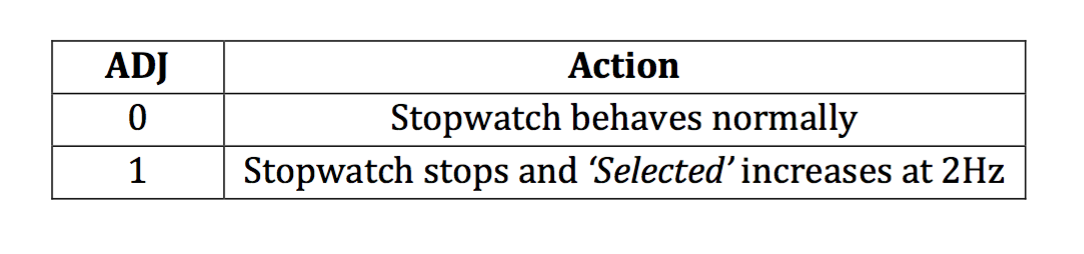
\includegraphics[width=14cm, height=3cm]{adj.png}
           % \captionof{figure}{Output Waveforms}
           % \label{fig:figure1}
        \end{minipage}
\item \textbf{SEL}:SEL is used to select which portion is incremented in adjustment mode.\\
\begin{minipage}{\linewidth}
            \centering
            
\includegraphics[width=14cm, height=2.2cm]{sel.png}
           % \captionof{figure}{Output Waveforms}
           % \label{fig:figure1}
        \end{minipage}
\end{itemize}


\section*{Design}
We have 5 modules that implement the entire design.
\subsection*{clock\_divider}
clock\_div is the module to produce 4 clock signals of different frequencies.
\begin{itemize}
\item \textbf{1HZ}: The clock for normal increments of seconds.
\item \textbf{2HZ}: The clock for the adjustment mode.
\item \textbf{5HZ}: The clock for the blinking of the digits in the adjustment mode.
\item \textbf{500HZ}: The clock for multiplexing changes to seven segment display. The anode cycles through the 4 digits and displays 1 of them every 1/500th of a second. Since the clock is really fast, human eyes can not detect the transition and can see all four digits. 
\end{itemize}
This module has the master clock signal(100MHZ) and reset as the input. We use four 32-bit registers as counters to calculate the signal. The code goes as follows(just shows how to produce 1HZ snippet):\\
\begin{minipage}{\linewidth}
            \centering
            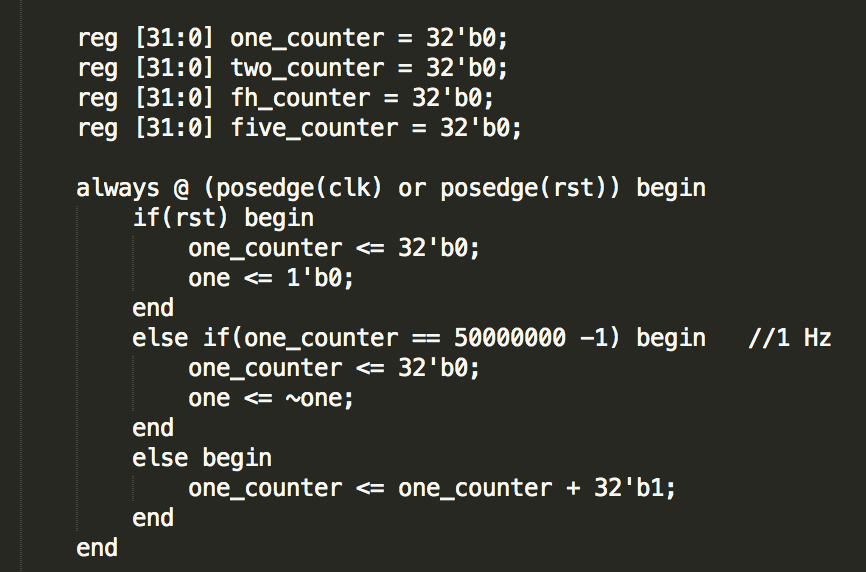
\includegraphics[width=14cm, height=5.9cm]{clock.png}
           % \captionof{figure}{Output Waveforms}
           % \label{fig:figure1}
        \end{minipage} 
Every 100000000(50000000*2) times, the signal changes from 0 to 1, thus generating the 1HZ signal.

\subsection*{counter}
This module is used to count the seconds and minutes. We use four 4-bit registers to record the changes of 4 digits(labeled as min1, min0, sec1, sec0). This module is implemented in 4 steps:
\begin{itemize}
\item The first step is to choose the correct clock signal. This module takes $adj$ as input to judge whether the watch is in adjustment mode. If $adj$ is 1, we choose 2HZ clock; else, we choose the normal 1HZ clock. 
\item The second step is to judge whether the watch is paused. If the watch is paused, no increments will happen.
\item When the clock is not in adjustment mode and is not paused, the counter begins to work normally. There are several special cases to consider. 
\begin{itemize}
\item If sec0 is 9 and sec1 is not 5, sec0 will be reset to 0 and sec1 increments by 1. 
\item If sec0 is 9 and sec1 is 5, we overflow into minutes sections and reset both sec0 and sec1 to 0. 
\item If min0 is 9 and min0 is not 5, min0 will be reset to 0 and min1 increments by 1. 
\item If min0 is 9 and min1 is 5, both min0 and min1 will be reset to 0.
\end{itemize}
Notice that the minute section increments only happen when seconds count up to 59. 
\item When the clock is in adjustment mode and not paused, we first use the input sel to find which portion will incremented. The edge cases are almost the same as the non-adjustment-mode ones. But this time we only need to take care of the selected digits. For example, when the clock shows 59:59 and the second digits are selected, the clock will become 59:00 instead of 00:00. No changes are made to minute digits.  

\end{itemize}

\subsection*{debouncer}
The buttons(reset and pause) need to be debounced because the unstable contact in FGPA board will bring some noise before a stable state. In order to obtain a stable state, a debouncer is needed to return a valid state of the button. \\
In this module, we take a 500HZ clock signal and the button signal as input. We create a 2-bit counter. If the button signal is 1, then the counter will increment by 1 on every rising edge of the clock. Once the counter reaches its maximum, it will output a valid state of the button. 

\subsection*{seven\_segment}
This module takes the binary representation of the digit(4-bit register) as input and outputs the 8-digit seven segment display.

\subsection*{stop\_watch}
This is the top module of our design. This module can be divided into these steps:
\begin{itemize}
\item Use the debouncer to get stable state of the reset and pause buttons.
\item Use clock\_divider to generate four clock signals for later use.
\item Use the counter to count the seconds and minutes.
\item Use seven\_segment to get the seven segment version of the digits. 
\item The last step is to control the final display of the four digits.
\begin{itemize}
\item First we need to control the anode of the seven segment display. Since there are 4 digits in total, we use a 2-bit register to select the digit. This register increments from 0 to 3; once it hits 3, it will be reset to 0. The anode varies from 0111 to 1110 in this process(from min1 to sec0).
\item Then we need to determine whether the clock is in adjustment mode and needs blinking. If adjust is set on, we need to buffer the clock display will blank with the blinking clock so that the selected fields will turn on and off at a blinking rate of 5HZ.
\end{itemize} 
This top module has two outputs: display and anode. Display is the seven segment of the digit chosen by anode, and anode itself is also needed for UCF file. 



\end{itemize} 

\begin{minipage}{\linewidth}
            \centering
            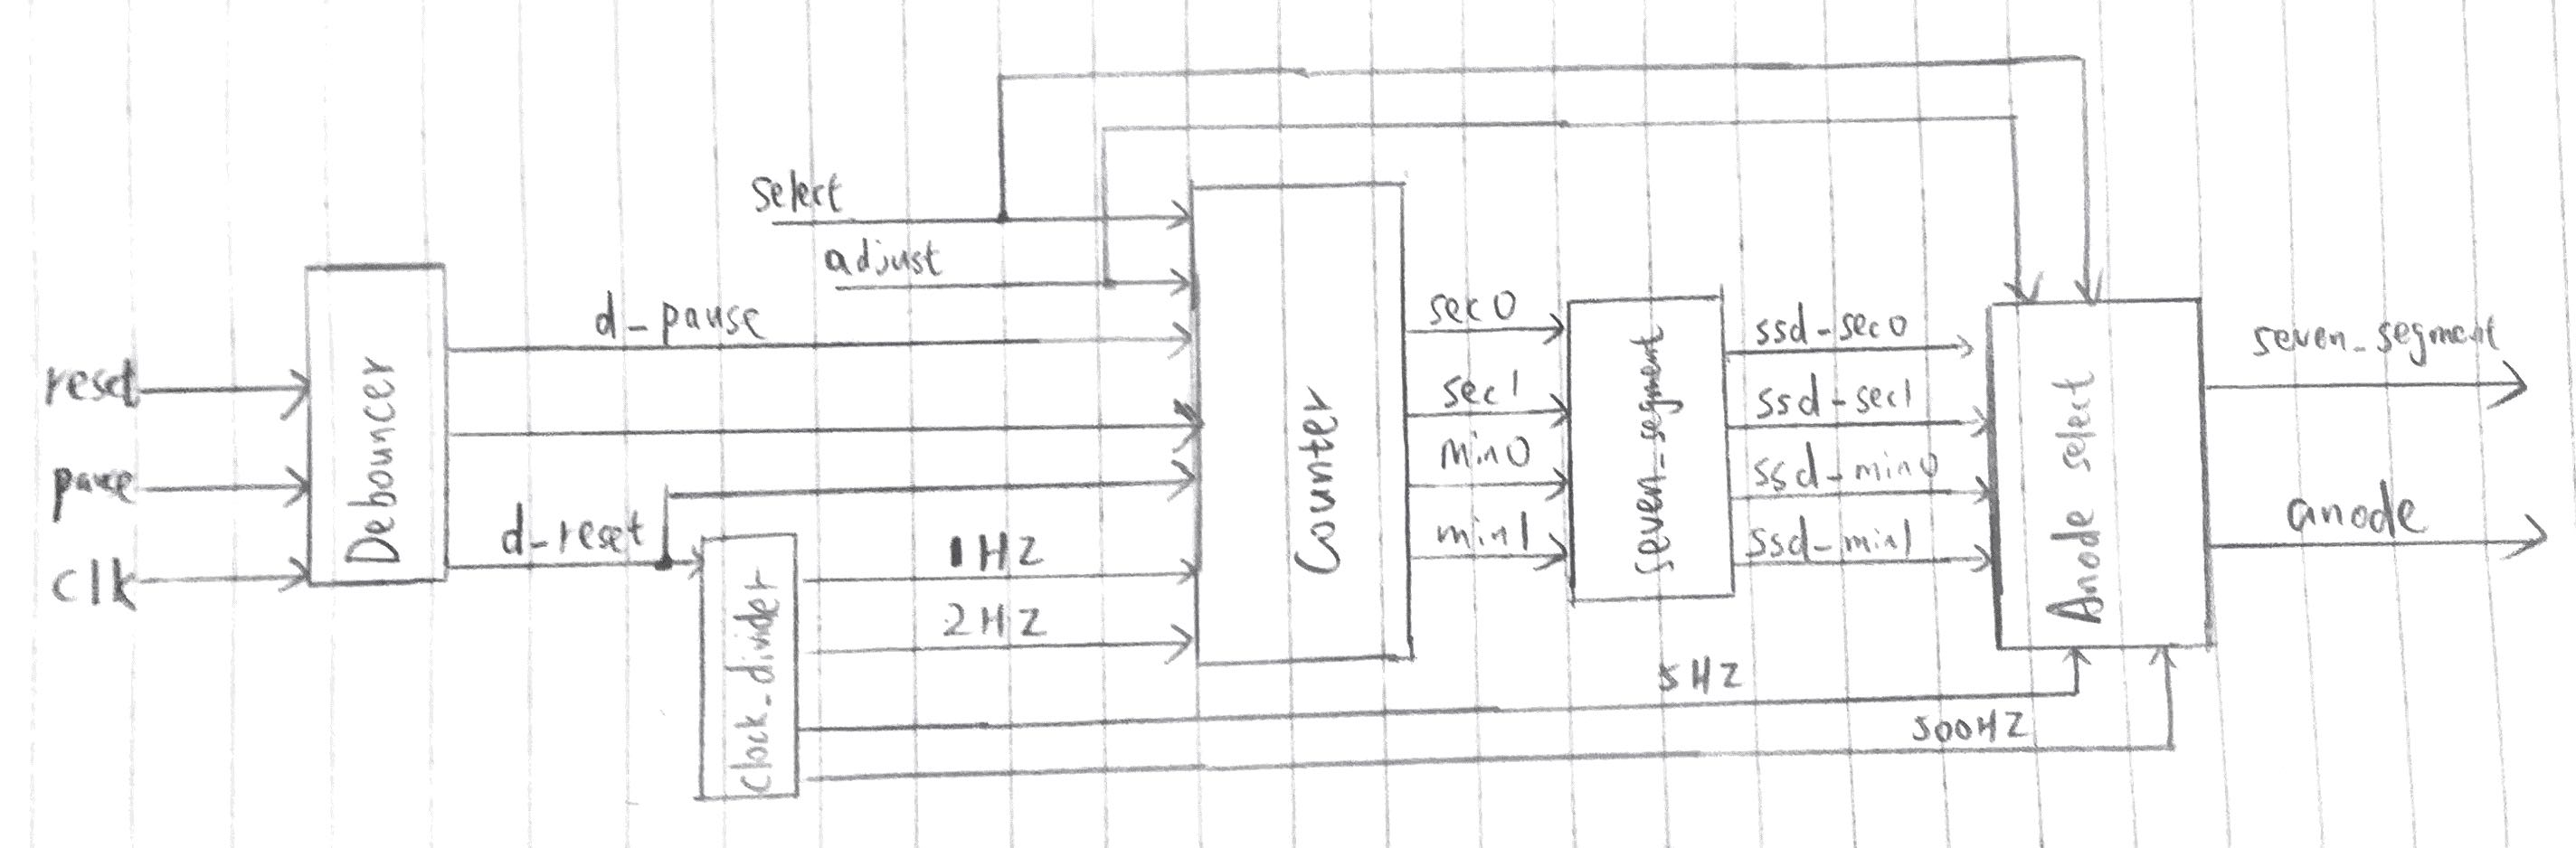
\includegraphics[width=15cm, height=5.9cm]{diagram.png}
            \captionof{figure}{Overall design diagram of stop watch}
            \label{fig:figure1}
        \end{minipage} 


\end{document}
